%% bulk_genome_comparisons_expt.tex
%% Author: Leighton Pritchard
%% Copyright: James Hutton Institute
%% Bulk genome comparisons - experimental

%
\begin{frame}
  \frametitle{Bulk genome comparisons}
  \Large{
    \textcolor{olive}{
      \textbf{
      You don't have to sequence genomes to compare them \\
      (but it helps) \\
      PART 1: Experimental
      }
    }
  }
\end{frame}

%
\begin{frame}
  \frametitle{Genome comparisons predate NGS}
  \begin{itemize}
    \item Sequence data wasn't always cheap and abundant
    \item Practical, experimental genome comparisons were needed
  \end{itemize}
  \begin{center}
    
\includegraphics[width=0.7\textwidth]{images/land_before_time}
  \end{center}  
\end{frame}

%
\begin{frame}
  \frametitle{Bulk genome comparisons}
  \Large{
    \textcolor{olive}{
      \textbf{
      Calculate values for individual genomes, \\
      then compare them.
      }
    }
  }
\end{frame}

%
\begin{frame}
  \frametitle{Bulk genome properties}
    \begin{itemize}
      \item Large-scale summary measurements
      \item Measure genomes independently - compare values later
        \begin{itemize}
         \item<2-2> \textcolor{red}{What kinds of measurements/properties?}
         \item<3-> \textcolor{hutton_green}{Number of chromosomes}
         \item<3-> \textcolor{hutton_blue}{Ploidy}
         \item<3-> \textcolor{RawSienna}{Chromosome size}
         \item<3-> \textcolor{hutton_purple}{Nucleotide (A,C,G,T) frequency}        
        \end{itemize}
    \end{itemize}
\end{frame}

%
\begin{frame}
  \frametitle{Chromosome stains
  \footnote{\tiny{\href{http://dx.doi.org/10.1038/nature03895
}{IRGSP (2005) \textit{Nature} doi:10.1038/nature03895
}}}
  \footnote{\tiny{\href{http://dx.doi.org/10.1038/nature11650
}{Brenchley \textit{et al}. (2012) \textit{Nature} doi:10.1038/nature11650
}}}
  }
  Count chromosomes, estimate size \\
  \textcolor{hutton_blue}{Wheat: 17Gbp; Rice: 390Mbp}
  \begin{center}
    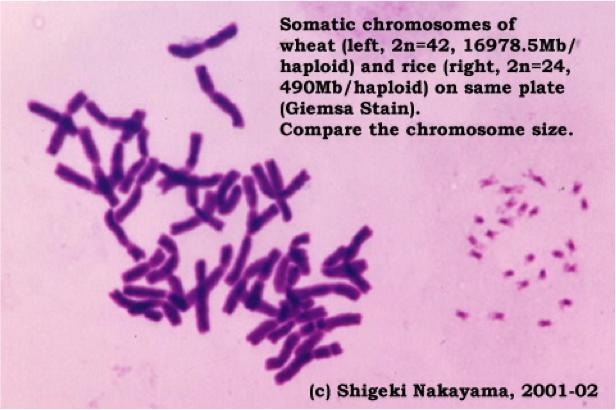
\includegraphics[width=0.7\textwidth]{images/wheat_rice_chromosomes}
  \end{center}  
\end{frame}

%
\begin{frame}
  \frametitle{Chromosome count/size
    \footnote{\tiny{Kamisugi \textit{et al}. (1993) \textit{Chromosome Res.} \textbf{1}(3): 189-196
}}
    \footnote{\tiny{\href{http://dx.doi.org/10.1038/nrg3375
}{Wang \textit{et al}. (2013) \textit{Nat. Rev. Genet.} doi:10.1038/nrg3375
}}}
  }
    \begin{itemize}
      \item \textcolor{hutton_green}{chromosome count and ploidy can vary widely} \\
        \begin{table}
		  \begin{tabular}{l | c | c }
		    Organism & Chromosomes & Ploidy  \\
			\hline \hline
			\textit{E. coli} & 1 & 1  \\ 
			Human (\textit{H. sapiens}) & 46 & 2 \\
			\hline
			Rice (\textit{O. sativa}) & 24 & 1  \\
			Adders-tongue & & \\ 
			(\textit{Ophioglossum reticulatum}) & 1260 & 84 \\
			\hline
			Domestic (not wild) wheat somatic & 42 & 6 \\
			Domestic (not wild) wheat gametic & 14 & 2 \\			
		  \end{tabular}
		\end{table}
	\end{itemize}
  \begin{center}
    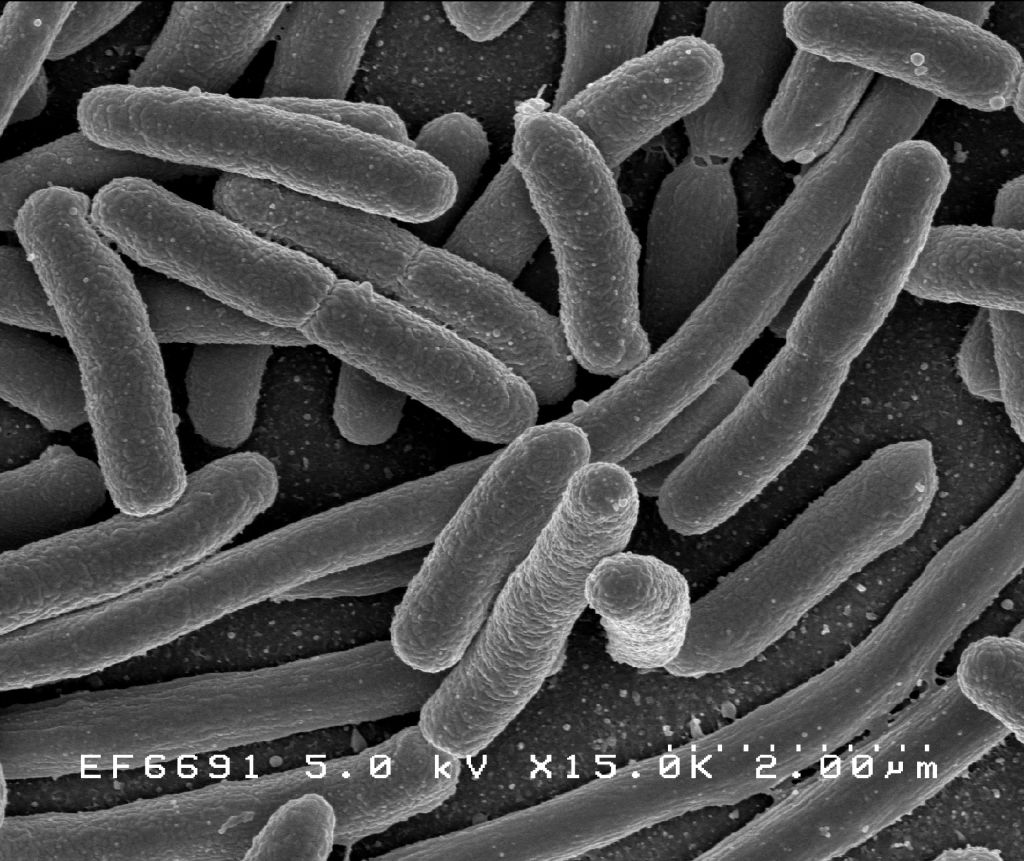
\includegraphics[height=0.15\textheight]{images/EscherichiaColi_NIAID}
    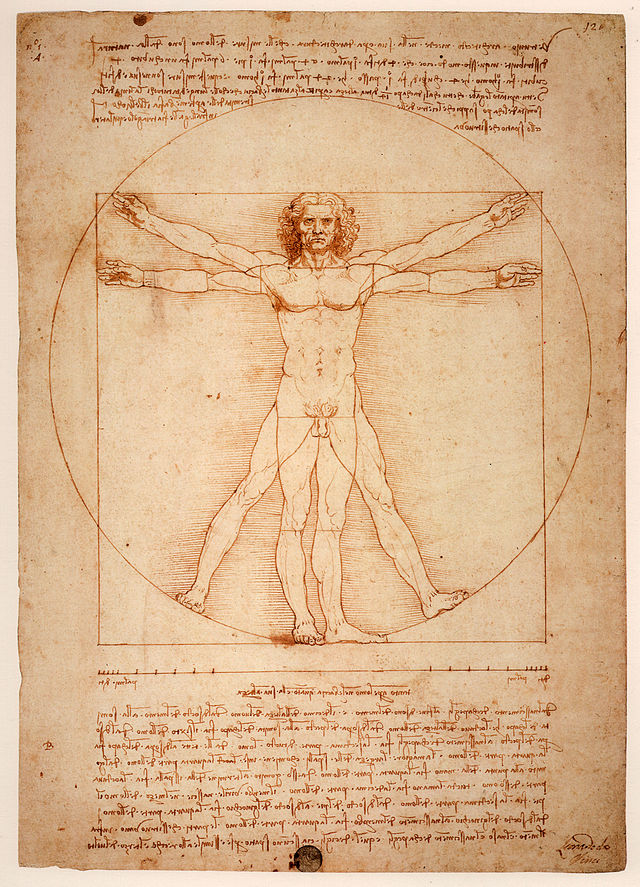
\includegraphics[height=0.15\textheight]{images/640px-Uomo_Vitruviano}
    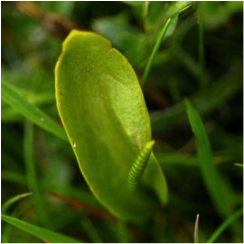
\includegraphics[height=0.15\textheight]{images/adders_tongue}
    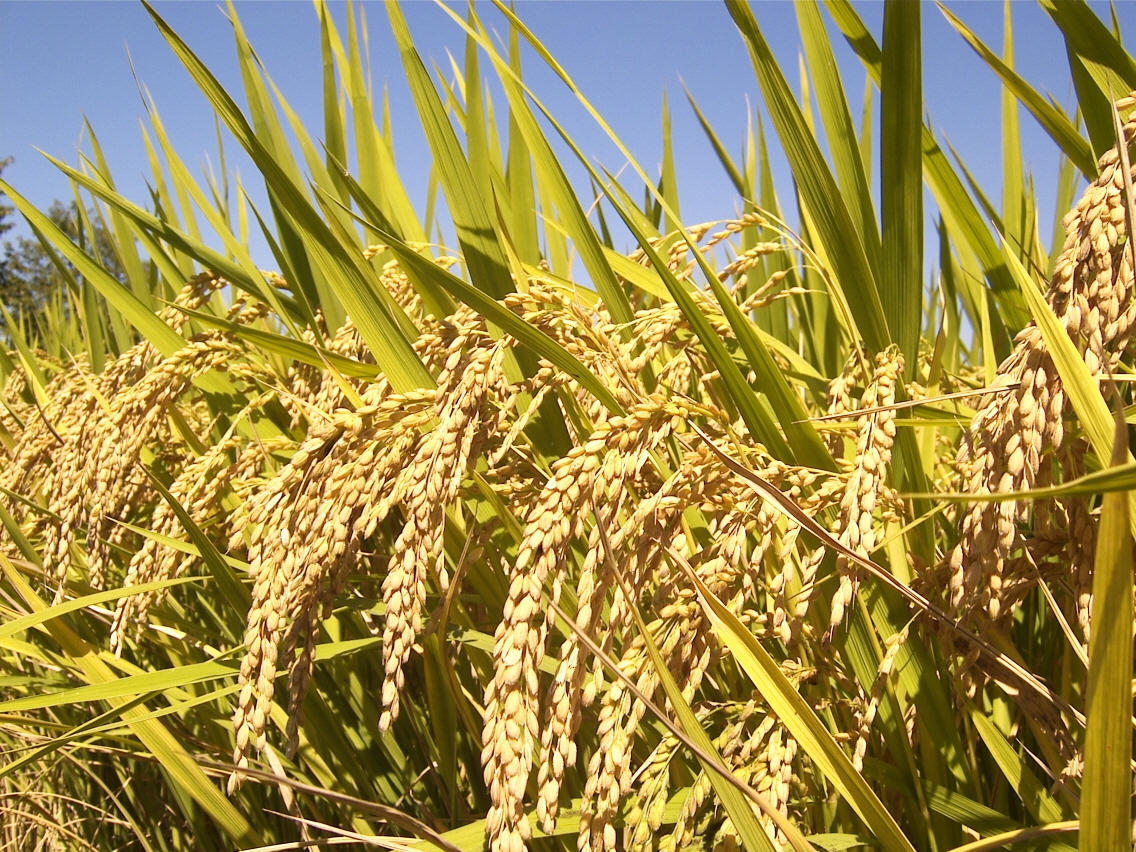
\includegraphics[height=0.15\textheight]{images/Rice_Plants_(IRRI)}
    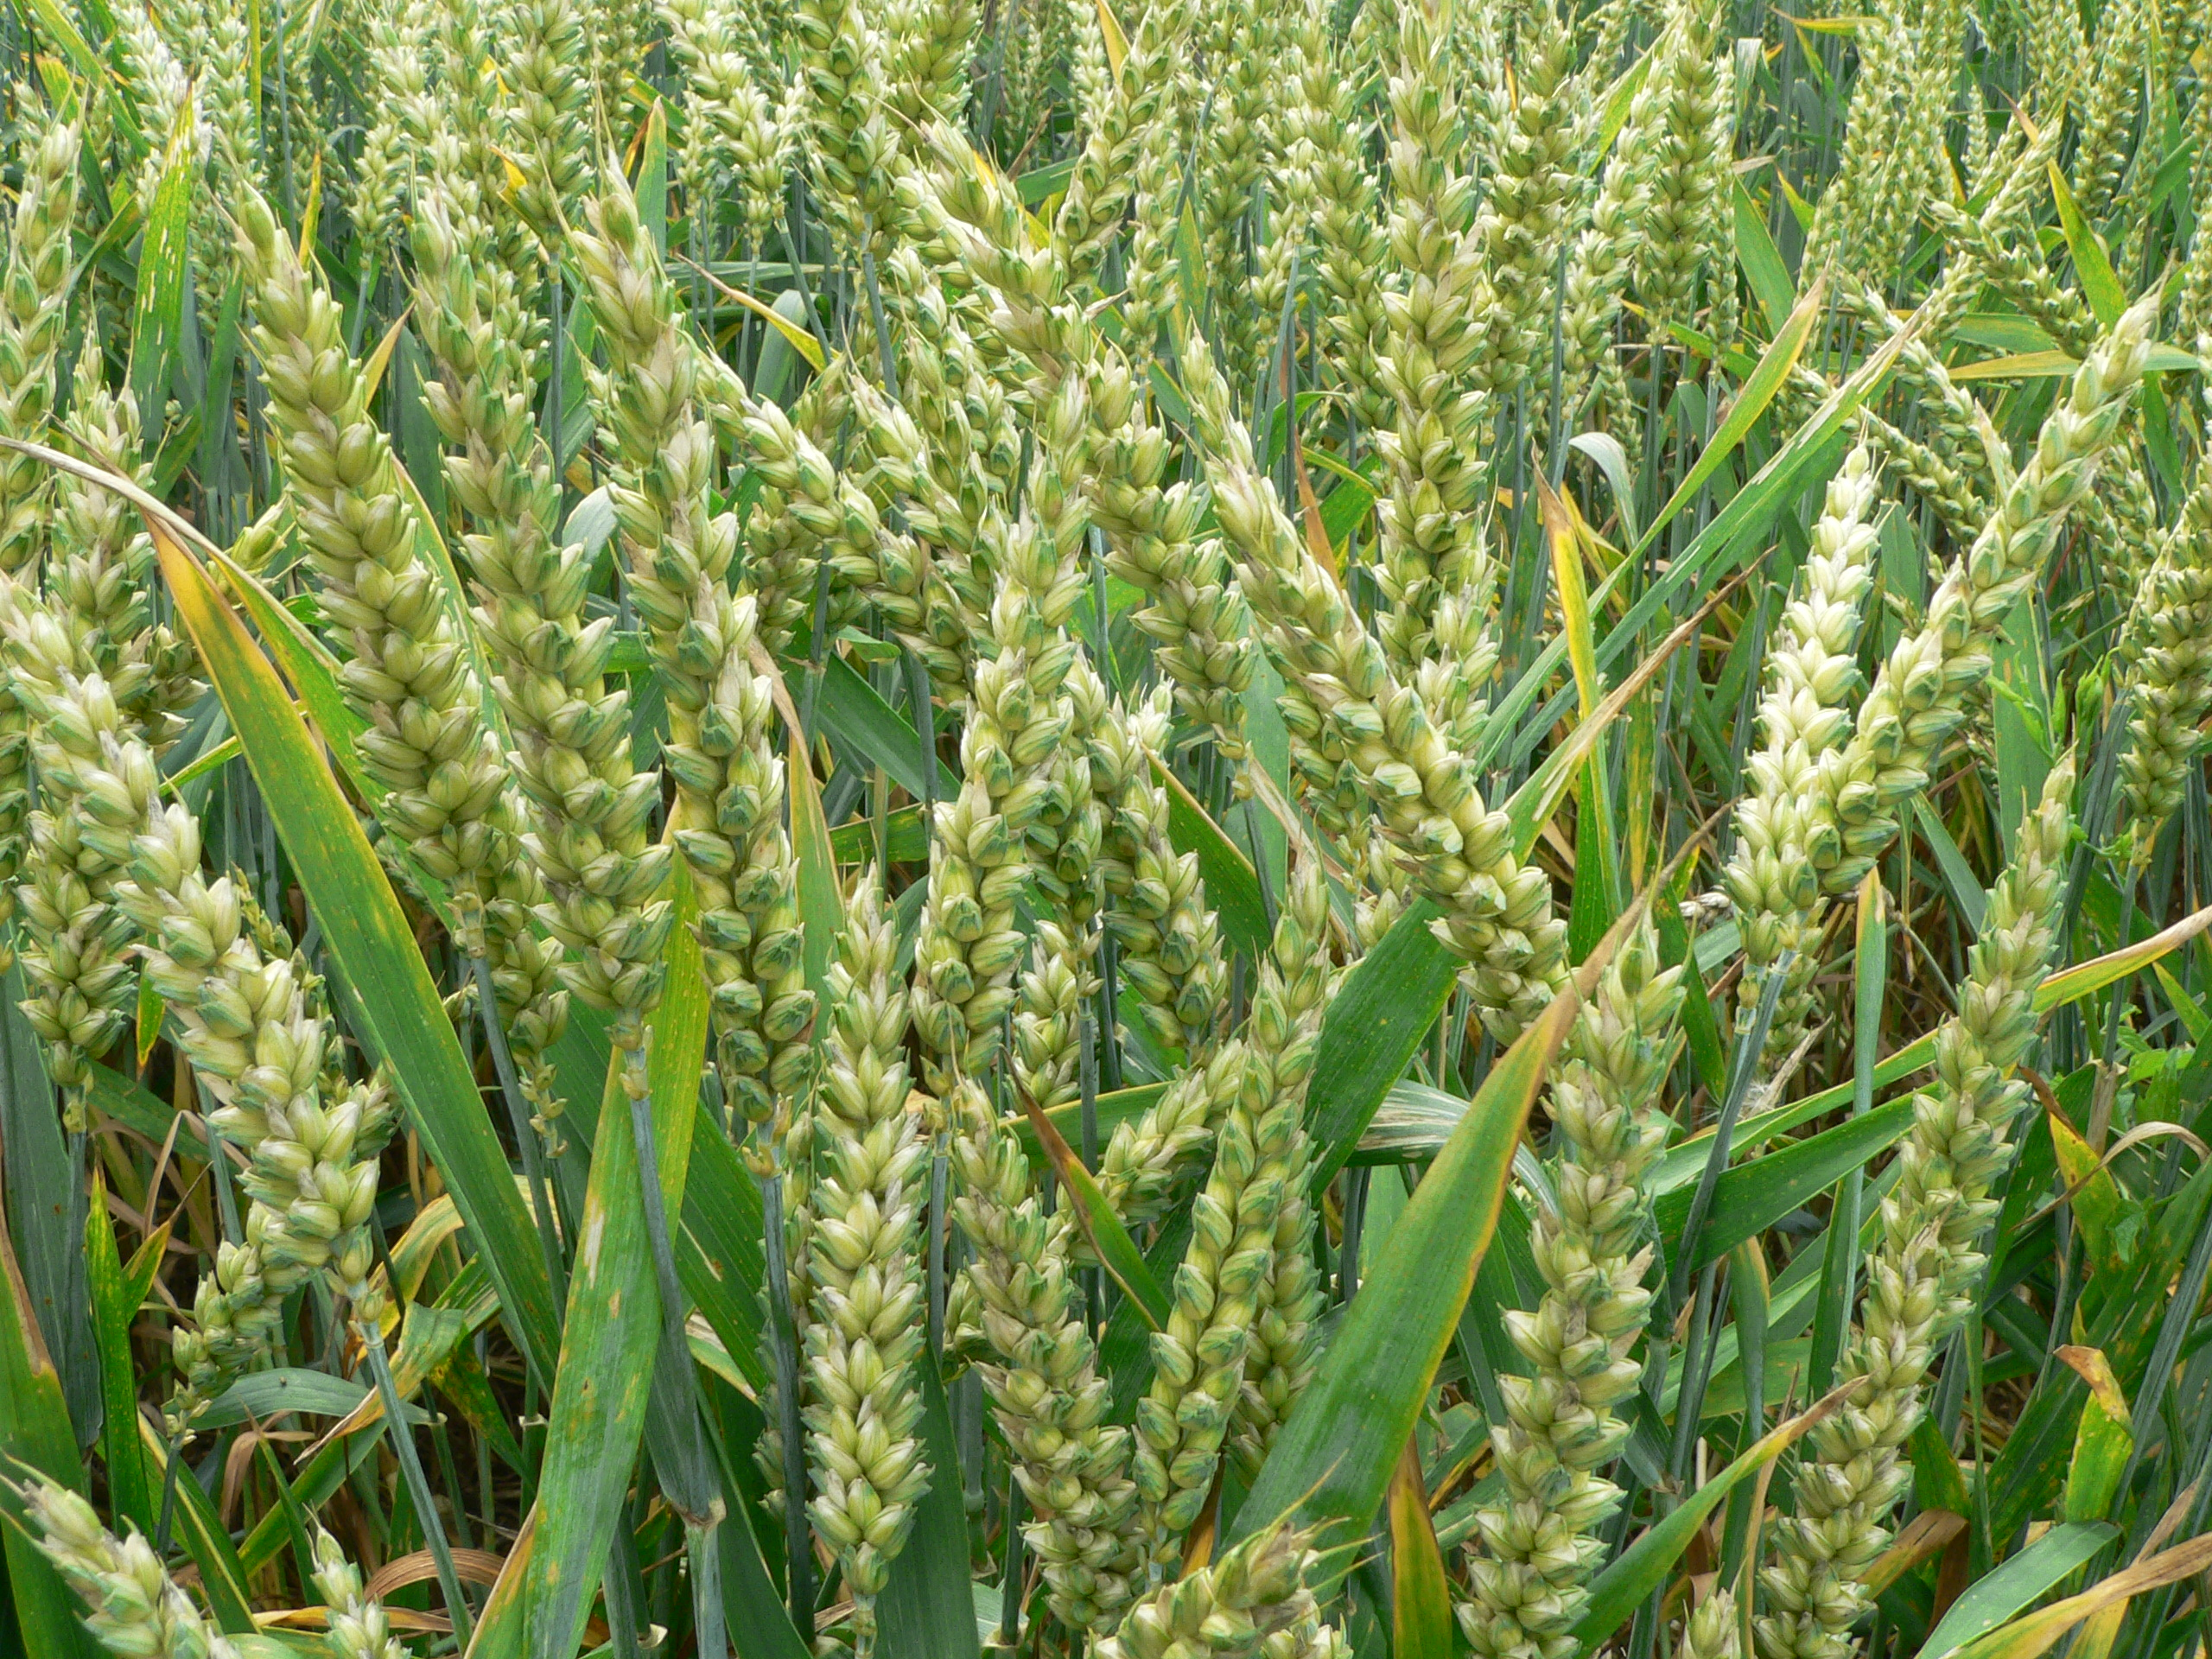
\includegraphics[height=0.15\textheight]{images/Wheat_P1210892}
  \end{center}  		
\end{frame}

%
\begin{frame}
  \frametitle{Physical study of chromosomes
  \footnote{\tiny{\href{http://dx.doi.org/10.1016/j.ymeth.2012.05.001
}{Belton \textit{et al}. (2012) \textit{Methods} doi:10.1016/j.ymeth.2012.05.001
}}}
  }
  \begin{itemize}
    \item \textcolor{hutton_green}{Genome size and chromosome count do \textbf{not} indicate organism ``complexity''}
    \item \textcolor{hutton_blue}{Modern physical study of chromosomes still produces surprises (e.g. Hi-C: chromatin interaction)}
  \end{itemize}
  \begin{center}
    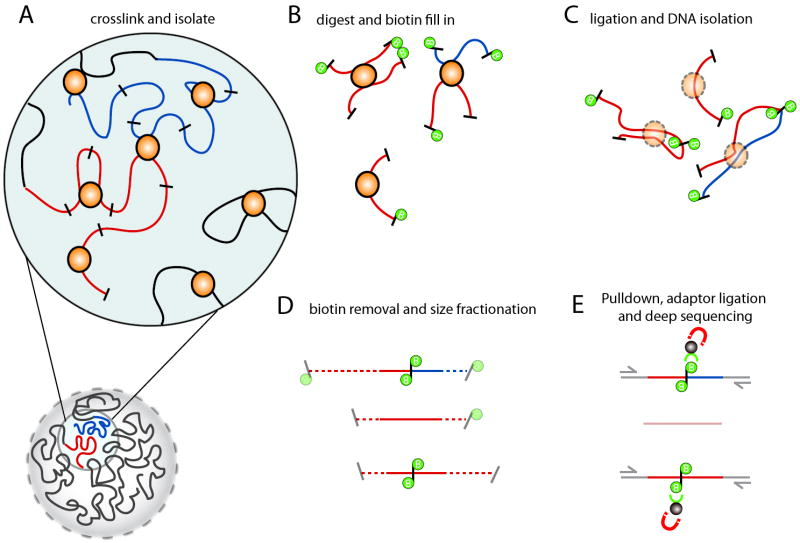
\includegraphics[width=0.7\textwidth]{images/nihms418977f1}
  \end{center}  
\end{frame}

%
\begin{frame}
  \frametitle{Nucleotide content
  \footnote{\tiny{Krane \textit{et al}. (1991) \textit{Nucl. Acids Res.} \textbf{19}(19): 5181-5185
}}
  }
  \begin{itemize}
    \item \textcolor{hutton_green}{Radiolabel monophosphates from genomic DNA}
    \item \textcolor{hutton_blue}{Separate by thin-layer chromatography}
    \item \textcolor{hutton_purple}{Compare label ratios using scanner}    
  \end{itemize}
  \begin{center}
    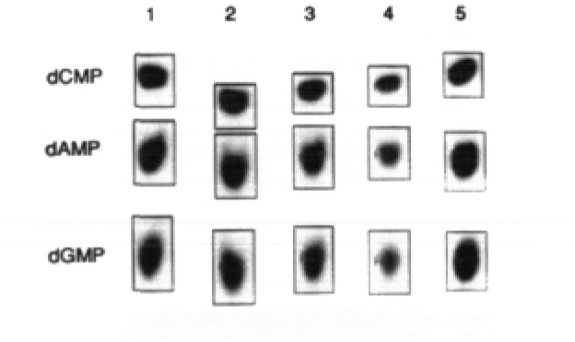
\includegraphics[height=0.4\textheight]{images/nucleotide_tlc}
    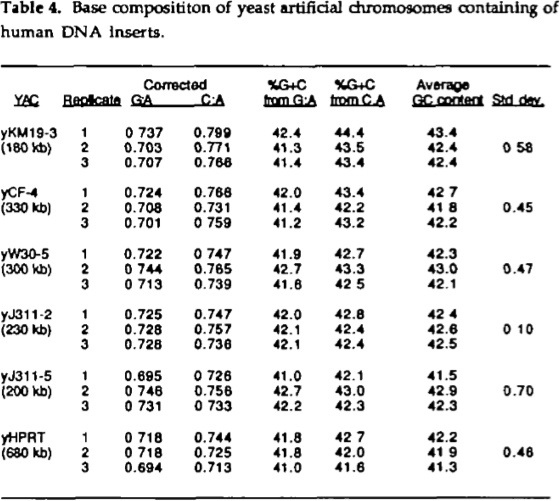
\includegraphics[height=0.4\textheight]{images/nucleotide_table}    
  \end{center}  
\end{frame}

%%
%\begin{frame}
%  \frametitle{Isochores
%  \footnote{\tiny{\href{http://dx.doi.org/10.1083/jcb.146.6.1211
%}{Sadoni \textit{et al}. (1999) \textit{J. Cell. Biol.} doi:10.1016/10.1083/jcb.146.6.1211
%}}}  
%  }
%    \begin{columns}[c] 
%      \column{.5\textwidth} 
%        \begin{itemize}
%         \item \textcolor{hutton_green}{ACGT composition varies within and between genomes}
%         \item \textcolor{RawSienna}{variation identified by staining}
%         \item \textcolor{hutton_blue}{\textit{isochore}: region with little internal GC variation}
%         \item \textcolor{hutton_purple}{In humans:}
%         \begin{itemize}
%           \item L1, L2: low GC ($\leq 41\%$)
%           \item H1, H2, H3: high GC ($\geq 41\%$)           
%         \end{itemize}
%        \end{itemize}
%      \column{.5\textwidth}
%        \begin{figure}
%        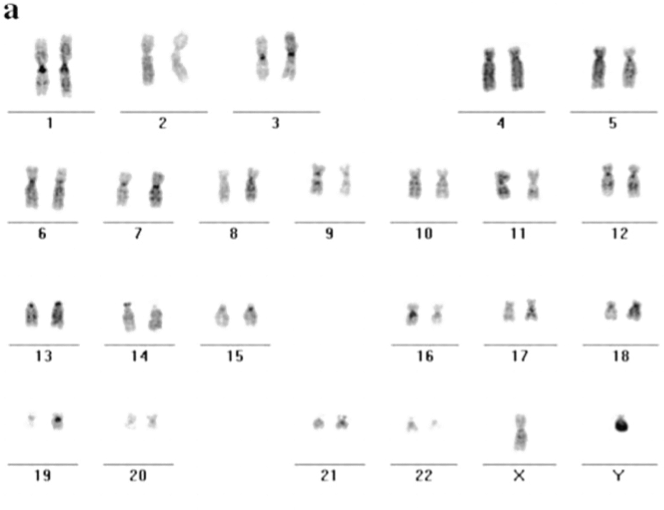
\includegraphics[width=\textwidth]{images/h3_isochores}
%        \caption{H3 isochore, human}
%        \end{figure}
%    \end{columns}  
%\end{frame}
